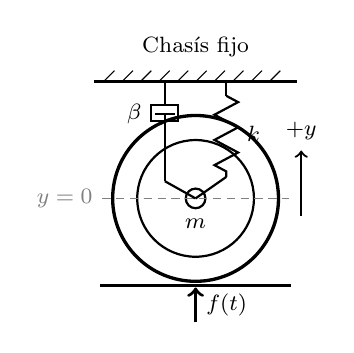
\begin{tikzpicture}[
  scale=0.78,
  every node/.style={font=\footnotesize},
  spring/.style={decorate,decoration={zigzag,segment length=3.2mm,amplitude=1.5mm}}
]
  % Chasís fijo
  \draw[very thick] (-1.65,1.90) -- (1.65,1.90);
  \foreach \x in {-1.5,-1.2,...,1.5}
    \draw[thin] (\x,1.90) -- ++(0.18,0.18);
  \node[anchor=south] at (0,2.15) {Chasís fijo};

  % Rueda y eje
  \draw[very thick] (0,0) circle (1.35);
  \draw[thick] (0,0) circle (0.95);
  \draw[fill=white,thick] (0,0) circle (0.16);
  \node[anchor=north] at (0,-0.18) {$m$};

  % Línea de equilibrio
  \draw[densely dashed,gray] (-1.52,0) -- (1.52,0);
  \node[anchor=east,gray] at (-1.52,0) {$y=0$};

  % Amortiguador
  \draw[thick] (-0.50,1.90) -- (-0.50,1.52);
  \draw[thick] (-0.72,1.26) rectangle (-0.28,1.52);
  \draw[thick] (-0.66,1.38) -- (-0.34,1.38);
  \draw[thick] (-0.50,1.38) -- (-0.50,0.28);
  \draw[thick] (-0.50,0.28) -- (0,0);
  \node[anchor=east] at (-0.72,1.38) {$\beta$};

  % Resorte
  \draw[thick] (0.50,1.90) -- (0.50,1.67);
  \draw[thick,spring] (0.50,1.67) -- (0.50,0.35);
  \draw[thick] (0.50,0.35) -- (0,0);
  \node[anchor=west] at (0.68,1.05) {$k$};

  % Suelo y fuerza
  \draw[very thick] (-1.55,-1.42) -- (1.55,-1.42);
  \draw[->,very thick] (0,-2.02) -- (0,-1.45)
    node[midway,right] {$f(t)$};

  % Coordenada positiva
  \draw[->,thick] (1.72,-0.28) -- (1.72,0.78)
    node[above] {$+y$};
\end{tikzpicture}

